% !TEX root = marvin.tex
\begin{figure*}[t]
  \begin{center}
  \iflatexml
    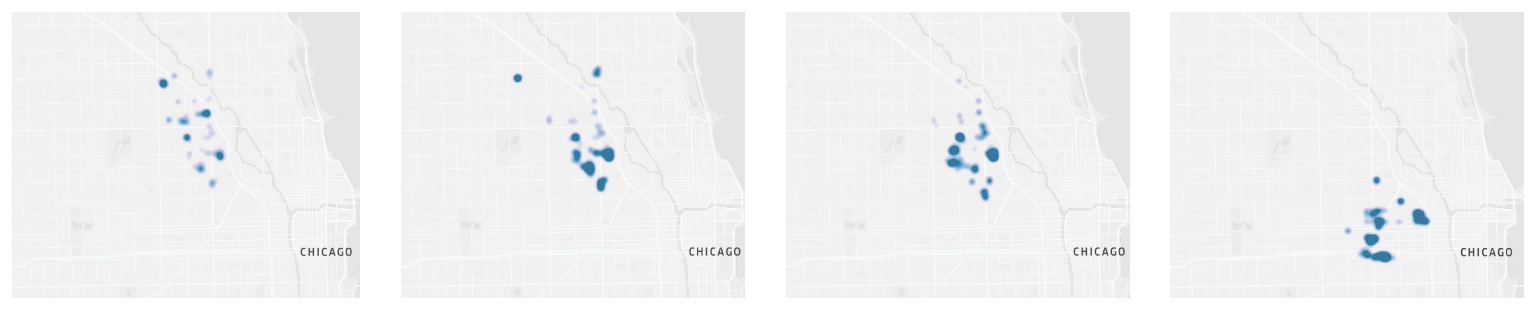
\includegraphics[width=6\textwidth]{figs/heatmap_spo.png}
  \else
    \begin{tabular}{llll}
      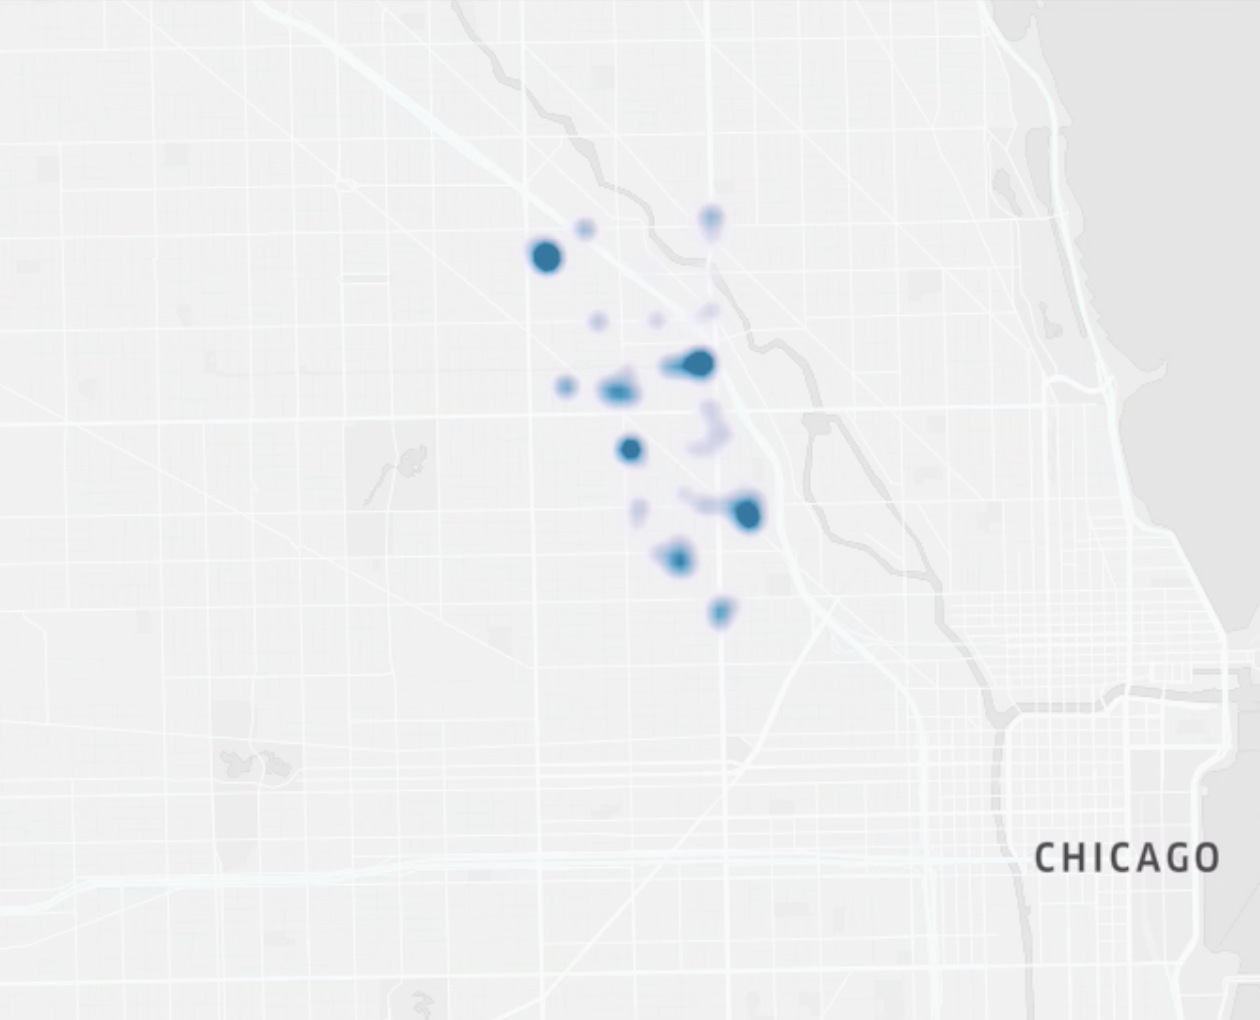
\includegraphics[height=3.0cm,trim={0.2cm 0 0.4cm 0},clip]{figs/sporadic1.png} &
      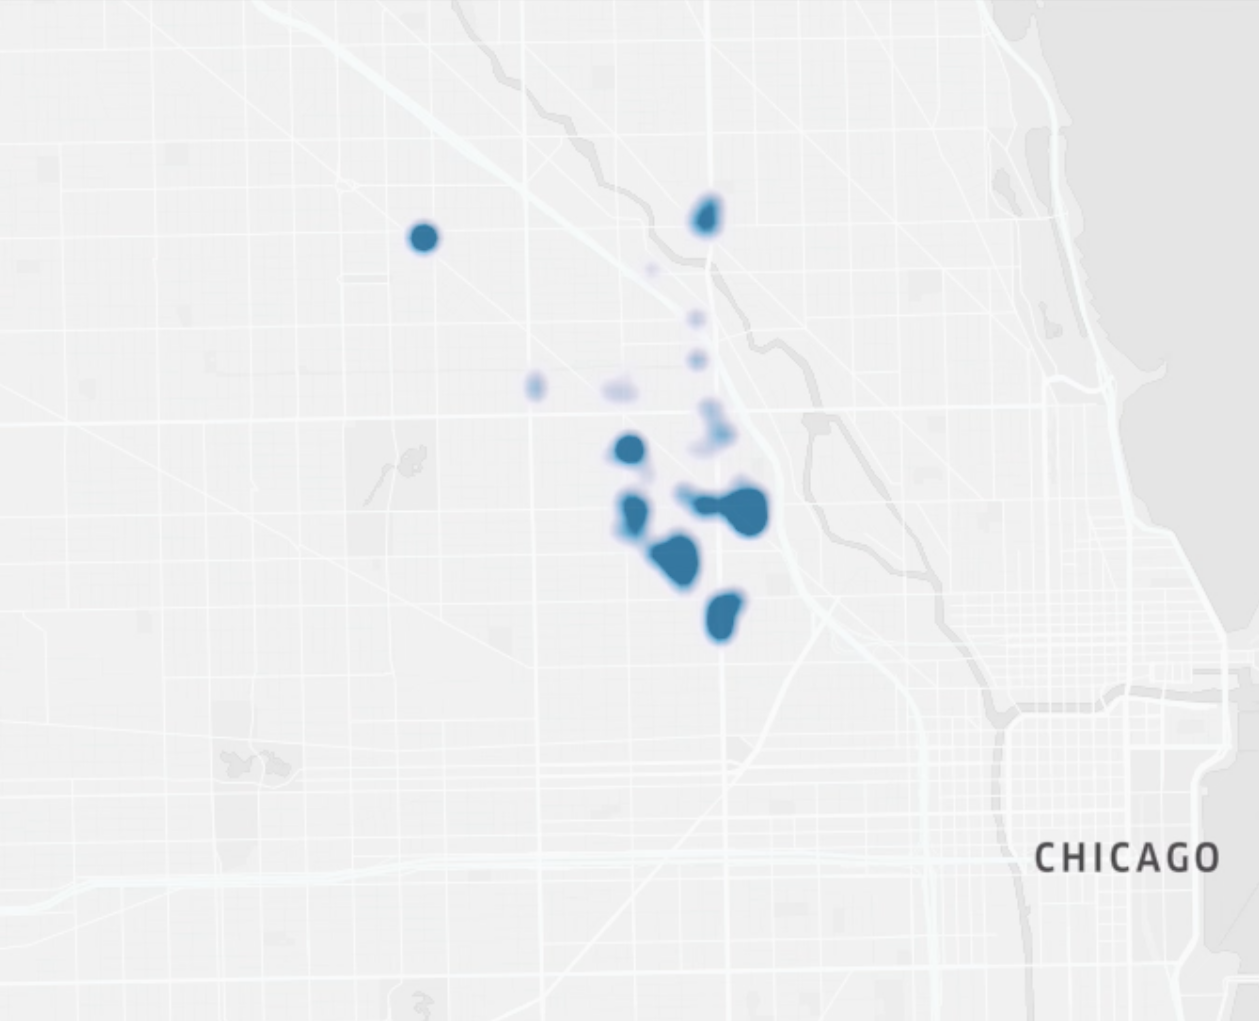
\includegraphics[height=3.0cm,trim={0.2cm 0 0.8cm 0},clip]{figs/sporadic2.png} &
      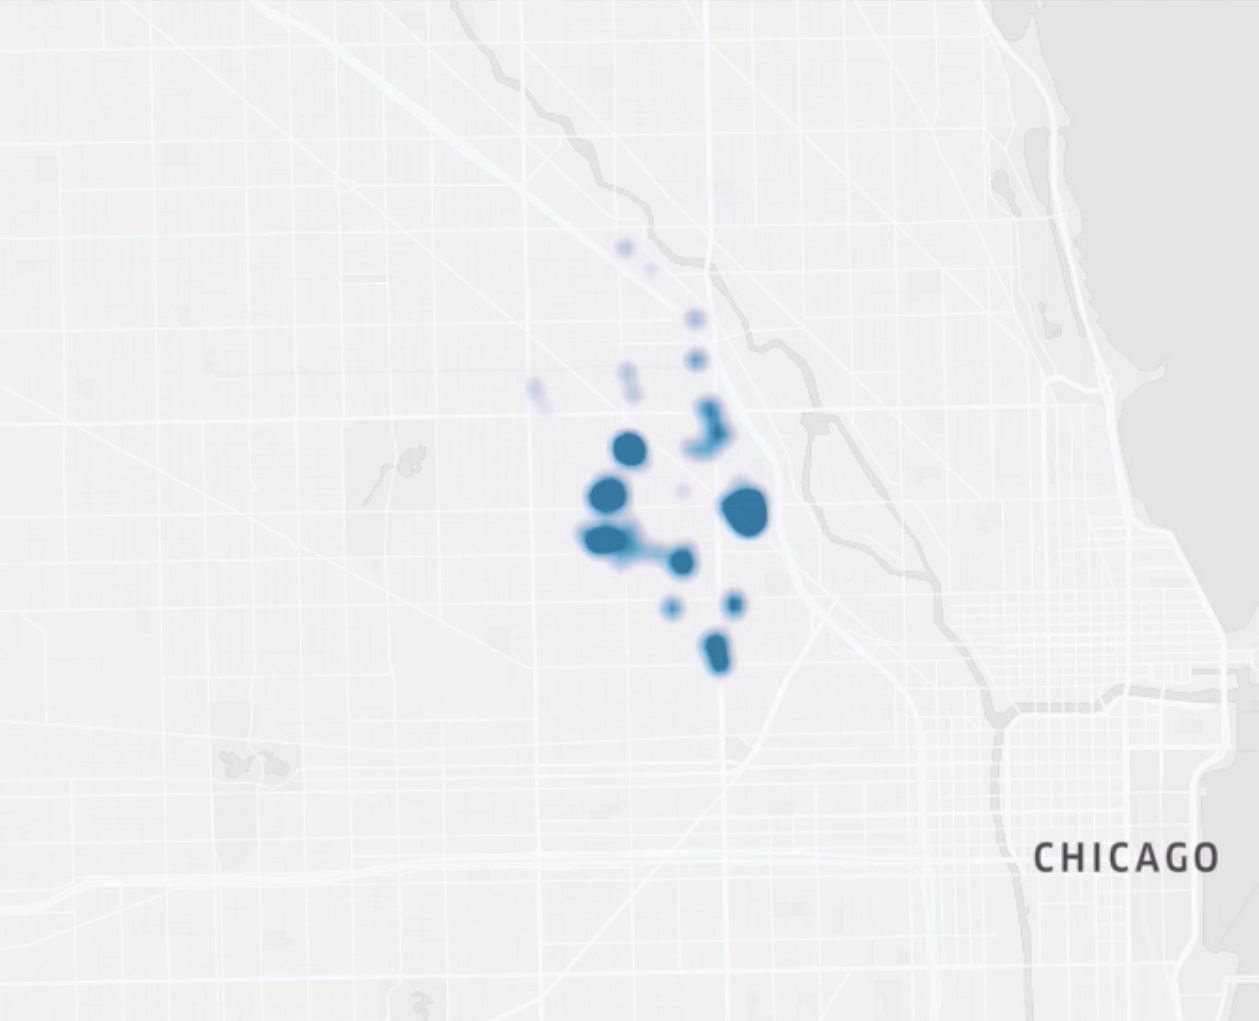
\includegraphics[height=3.0cm,trim={0.2cm 0 0.8cm 0},clip]{figs/sporadic3.png} &
      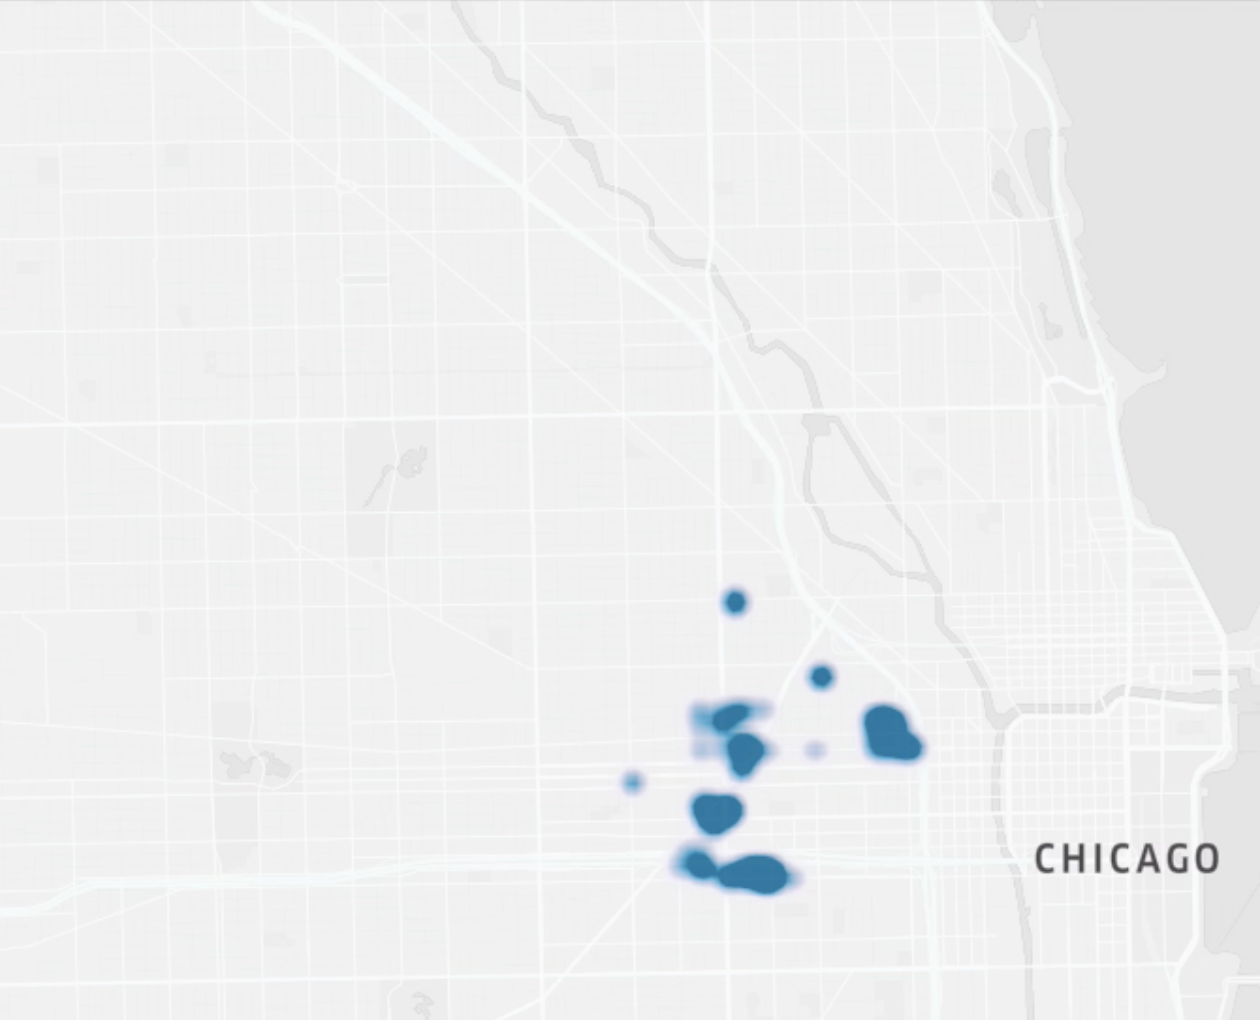
\includegraphics[height=3.0cm,trim={0.0cm 0 0cm 0},clip]{figs/sporadic4.png} \\
    \end{tabular}
  \fi
  % \vspace{-0.15in}
  \caption{Value function of an agents while mapping a given region.
  The value function is high around the roads that are distant and sporadically
  distributed implying an exploratory strategy. The red dot on the left and the blue dot
  on the right represent the agent's current position.}
  \label{fig:heatmap_sporadic}
  \end{center}
  \vspace{-0.25in}
\end{figure*}